\section{Ordinary Least Squares}
This section will introduce the method of ordinary least squares for estimating parameters in a multiple linear regression model.
The first section however will motivate the method of ordinary least squares through an example of simple linear regression.

\subsection{Least Squares}
The purpose of using the least squares method is minimizing the sum of squared residuals, also known as $SSR$.
Residuals refers to the difference between the observed and fitted values.
Given a set of data points in the plane, how might one find the line that best fit the data? 
One way is to choose the line that minimizes the sum of squared residuals.
In figure \ref{fig:example_simple_linear_regression} an example of a simple linear regression can be seen. 
The figure illustrates the log price plotted against the construction year of apartments sold by HOME in Aalborg within the year 2012.

\begin{figure}[h]
    \centering
    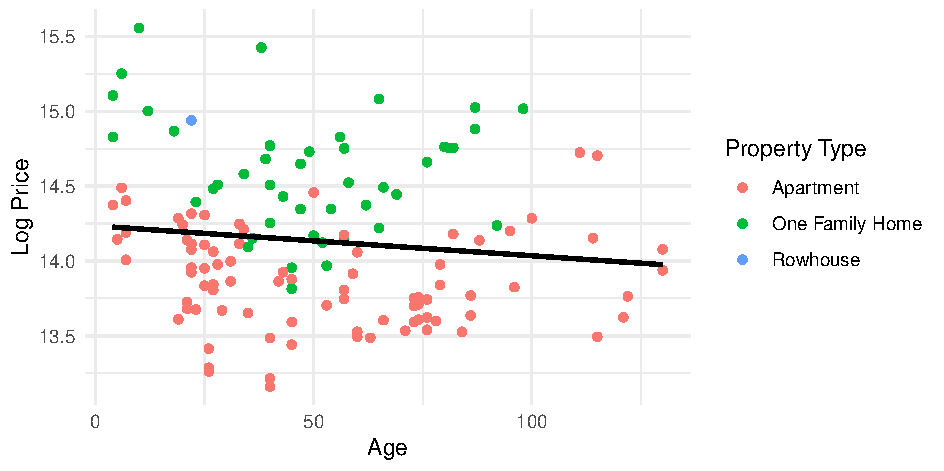
\includegraphics[width = 0.9\textwidth]{figures/Ordinary_Least_Squares/example_linear_regression.pdf}
    \caption{Construction year and $\log(price)$ of apartments sold in 2012 by Home in Aalborg.}
    \label{fig:example_simple_linear_regression}
\end{figure}

The data set has observations $\{a_i, log(p_i)\}$ with $i = 1, \ldots, 27$. 
The construction year of the property is seen as the independent variable and the log price as the dependent variable.
We can assume that there is a linear relationship between construction year and log price of the property in question.
This can be formulated as
\begin{align}\label{eq:approx_linear_relationship}
    \log(p) \approx \beta_0 + \beta_1 a
\end{align}
where $log(p)$ and $a$ denotes the log price and construction year respectively.
The right side \eqref{eq:approx_linear_relationship} is the model function in our case.
The function is on the form $f(a, \betabold)$, where $\betabold$ is a $2 \times 1$ vector containing the coefficients $\beta_0$ and $\beta_1$.
The goal is now to find $\betabold$ that minimizes the sum of squared residuals.
For the $i$'th observation the residual is defined as $r_i = \log(p_i) - f(a_i, \betabold)$.
With the notation in place we can now write the sum of squared residuals as
\begin{align}
  SSR(\betabold) = \sum_{i = 1}^{27} r_i^2 &= \sum_{i = 1}^{27} \left( \log(p_i) - f(a_i, \betabold) \right)^2 \nonumber\\
  &= \sum_{i = 1}^{27} \left( \log(p_i) - (\beta_0 + \beta_1 a_i) \right)^2.\label{eq:SSR}
\end{align}
The line that best fit the data is given by the $\betabold$ that minimizes \eqref{eq:SSR} over all possible values $\betabold$.
In the next section this optimization problem will be formulated with matrix notation.
The intuition provided here, using simple linear regression, can then be used in the case of multiple linear regression.
In the mean time the regression of log price on construction year performed by \texttt{R} is shown in the table below.
\begin{table}[H]
    \centering
    \begin{tabular}{lrrrr}
        \toprule
        \textbf{term} & \textbf{estimate} & \textbf{std.error} & \textbf{\textit{t}-statistic} & \textbf{p.value}\\
        \midrule
        Intercept & 14.887515 & 0.316951 & 46.971 & 0.00000\\
        year.construct & -0.007668 & 0.002325 & -3.298 & 0.00292\\
        \bottomrule
    \end{tabular}
    \caption{Regression coefficients from regressing $\log(price)$ on year.construct.}
    \label{tab:regress_log_price_on_age}
\end{table}
In table \ref{tab:regress_log_price_on_age} intercept refers to $\beta_0$ and construction year coefficient refers to $\beta_1$.
As $\beta_1$ is negative the data indicates a slight negative relationship between log price and construction year.
As the $p$ value is below 0.05 the relationship is regarded as statistically significant on a 95\% confidence level.
To fully grasp this concept, the concept of hypothesis testing will be introduced in chapter \ref{ch:hypothesis_testing}.

\subsection{Parameter Estimation in Matrix Form}
Estimating parameters for a multiple linear regression model in case of matrix notation still translates to minimizing the sum of squared residuals, but the model function for the $i$'th observation can now be rewritten as
\begin{align*}
    \beta_0 + x_{i1} \beta_1 + \cdots + x_{ik}\beta_k =
    \begin{bmatrix} 
    1 & x_{i1} & \cdots & x_{ik}  
    \end{bmatrix} 
    \begin{bmatrix}
    \beta_0 \\ \beta_1 \\ \vdots \\ \beta_k
    \end{bmatrix} = \mathbf{x}_i \boldsymbol{\beta}.
\end{align*}
Where $\mathbf{x}_i$ denotes the $i$'th row in the design matrix $\mathbf{X}$.
Thus the sum of squared residuals is given by
\begin{align*}
    SSR(\boldsymbol{\beta}) = \nsum (y_i - \mathbf{x}_i\boldsymbol{\beta})^2.
\end{align*}
% where $y_i$ denotes the price of property $i$ and $\mathbf{x}_i$ denotes the $i$'th row in the design matrix $\mathbf{X}$.
Suppose that $\betahat$ minimizes the sum of squared residuals, that is
\begin{align*}
    \betahat = \underset{\boldsymbol{\beta}}{\argmin} \nsum (y_i - \mathbf{x}_i\boldsymbol{\beta})^2.
\end{align*}
Where arg is the argument that minimizes the $SSR$ w.r.t.$\!$ $\boldsymbol{\beta}$. Then $\betahat$ must satisfy the condition $\nabla \ssr(\betahat) = 0$.
Taking the derivative w.r.t. $\boldsymbol{\beta}$ yields
\begin{align}\label{eq:ssr_derivative}
    \frac{\partial SSR(\boldsymbol{\beta})}{\partial \boldsymbol{\beta}} 
    =  \nsum -2(y_i - \mathbf{x}_i \boldsymbol{\beta})\mathbf{x}_i.
\end{align}
The expression $\nabla \ssr (\betahat) = 0$ can now be rewritten as
\begin{align*}
    \nsum -2(y_i - \mathbf{x}_i \betahat)\mathbf{x}_i = \mathbf{0} 
    \quad \Rightarrow \quad
    \nsum \mathbf{x}_i^\top(y_i - \mathbf{x}_i \betahat) = \mathbf{0}
\end{align*}
by taking the transpose and dividing by $-2$.
The condition is now a vector of size $(k + 1) \times 1$ and thus represents a system of $k + 1$ equations with $k + 1$ unknowns.
Writing the vector as a system of equations gives the following $k + 1$ equations
\begin{align}\label{eq:multiple_linear_regression_equations}
\begin{split}
    \nsum (y_i - \betahat_0 -  \mathbf{x}_{i1} \betahat_1 - \cdots - \betahat_k \mathbf{x}_{ik}) &= 0 \\
    \nsum \mathbf{x}_{i1}(y_i - \betahat_0 -  \mathbf{x}_{i1} \betahat_1 - \cdots - \betahat_k \mathbf{x}_{ik}) &= 0 \\
    &\vdots \\
    \nsum \mathbf{x}_{ik}(y_i - \betahat_0 -  \mathbf{x}_{i1} \betahat_1 - \cdots - \betahat_k \mathbf{x}_{ik}) &= 0.
\end{split}
\end{align}
Returning to the notation used in \eqref{eq:multiple_linear_regression_model}, \eqref{eq:multiple_linear_regression_equations} will now be rewritten to matrix notation
\begin{align}
    \mathbf{X}^\top(\mathbf{y} - \mathbf{X}\betahat) &= \mathbf{0} \nonumber\\
    \mathbf{X}^\top\mathbf{y} - \mathbf{X}^\top\mathbf{X}\betahat &= \mathbf{0}\nonumber\\
    \mathbf{X}^\top\mathbf{X}\betahat &= \mathbf{X}^\top\mathbf{y}\label{eq:equation_from} \\
    \betahat &= \left(\mathbf{X}^\top\mathbf{X}\right)^{-1}\mathbf{X}^\top\mathbf{y}. \label{eq:equation_to}
\end{align}

Going from \eqref{eq:equation_from} to \eqref{eq:equation_to} one must assume that $\mathbf{X}^\top\mathbf{X}$ is positive definite and thereby invertible.
It turns out that this is not the only assumption we have to make, there are in fact four assumptions related to the OLS estimator.
Together these assumptions are known as the Gauss-Markov assumptions. 
They will now be introduced.
\begin{assumption}[Linear in parameters]\label{as:linear_in_the_parameters}
    The model can be written as $\mathbf{y} = \mathbf{X}\boldsymbol{\beta} + \boldsymbol{\varepsilon}$ where $\mathbf{y}$ is an observed $n \times 1$ vector, $\mathbf{X}$ is an $n \times (k + 1)$ observed matrix, and $\boldsymbol{\varepsilon}$ is an $n \times 1$ vector of unobserved errors or disturbances.
\end{assumption}
\begin{assumption}[No perfect collinearity]\label{as:no_perfect_collinearity}
    The matrix $\mathbf{X}$ has full column rank.
\end{assumption}
As the design matrix $\mathbf{X}$ has $n$ rows and $k + 1$ columns, assumption \ref{as:no_perfect_collinearity} implies that $n \geq k + 1$.
Moreover it implies that $\mathbf{X}$ has full column rank and thereby that $\mathbf{X}^\top\mathbf{X}$ is positive definite.
To prove this consider an arbitrary matrix $\textbf{A}$ of size $m \times n$.
The matrix $(\textbf{A}^\top \textbf{A})$ is symmetric and positive semi definite, as for any $\textbf{v} \in \mathbb{R}^n$
\begin{align}\label{eq:positive_semi_definite}
\textbf{v}^\top (\textbf{A}^\top \textbf{A}) \textbf{v} = (\textbf{v}^\top \textbf{A}^\top) (\textbf{A} \textbf{v}) = (\textbf{A} \textbf{v})^\top (\textbf{A} \textbf{v}) \geq 0.
\end{align}
Assume now that $\textbf{A}$ has rank $n$ and for contradiction that $\textbf{v}^\top \textbf{A} \textbf{v} = 0$.
By \eqref{eq:positive_semi_definite} this is a contradiction as it would imply that $\textbf{vA} = \textbf{0}$ which cannot be true for a matrix of full column rank.
This is because a matrix of full column rank has columns that are linearly independent.
Thus it is proven that if $\textbf{A}$ has full column rank then $\textbf{A}^\top \textbf{A}$ is positive definite.
\begin{assumption}[Zero conditional mean]\label{as:zero_conditional_mean}
    Conditional on the entire matrix $\mathbf{X}$, each residual $\varepsilon_i$ has zero mean, i.e. \cite[p. 810]{Wooldridge2012}
    \begin{align*}
        E(\varepsilon_i | \mathbf{X}) = 0, \quad i = 1, 2, \ldots, n.
    \end{align*}
\end{assumption}
This assumption ensures that there is no correlation between each of the explanatory variables and $\varepsilon_i$ for $i = 1, \ldots, n$.
If it on the other hand was the case that $x_j$ were correlated with $\varepsilon_i$, the explanatory variable would be called an endogenous explanatory variable.
In the case that assumption \ref{as:zero_conditional_mean} holds and thereby that none of the explanatory variables are correlated with $\varepsilon_i$, we have what is called exogenous explanatory variables.
\begin{theorem}[Unbiasedness of OLS]\label{th:unbiasedness_of_ols}
    Under assumptions \ref{as:linear_in_the_parameters}, \ref{as:no_perfect_collinearity} and \ref{as:zero_conditional_mean}, the OLS estimator $\betahat$ is an unbiased estimator for $\boldsymbol{\beta}$ \cite[p. 810]{Wooldridge2012}.
\end{theorem}
\begin{proof}
    Under assumptions \ref{as:linear_in_the_parameters} and \ref{as:no_perfect_collinearity} we can write $\betahat$ as
    \begin{align}
        \betahat &= (\mathbf{X}^\top\mathbf{X})^{-1}\mathbf{X}^\top\mathbf{y} \nonumber\\
        &= (\mathbf{X}^\top\mathbf{X})^{-1}\mathbf{X}^\top(\mathbf{X}\boldsymbol{\beta} + \boldsymbol{\varepsilon}) \nonumber\\
        &=(\mathbf{X}^\top\mathbf{X})^{-1}\mathbf{X}^\top\mathbf{X}\boldsymbol{\beta} + (\mathbf{X}^\top\mathbf{X})^{-1}\mathbf{X}^\top\boldsymbol{\varepsilon} \nonumber\\
        &= \boldsymbol{\beta} + (\mathbf{X}^\top\mathbf{X})^{-1}\mathbf{X}^\top\boldsymbol{\varepsilon} \label{eq:beta_hat_unbiased}
    \end{align}
    Taking the conditional expectation of \eqref{eq:beta_hat_unbiased} on $\mathbf{X}$ and using the fact that $E(\boldsymbol{\varepsilon} | \mathbf{X}) = 0$ gives
    \begin{align*}
        E(\betahat | \mathbf{X}) &= \boldsymbol{\beta} + (\mathbf{X}^\top\mathbf{X})^{-1}\mathbf{X}^\top E(\boldsymbol{\varepsilon} | \mathbf{X}) \\
        &= \boldsymbol{\beta} + (\mathbf{X}^\top\mathbf{X})^{-1}\mathbf{X}^\top \mathbf{0} \\
        &= \boldsymbol{\beta}
    \end{align*}
    It is now shown that $\betahat$ is unbiased as defined in definition \ref{def:Unbiased_estmator} on page \pageref{def:Unbiased_estmator}.
\end{proof}

\subsection{Homoskedasticity and Heteroskedasticity}

In order to state the next assumption, we need a definition that enables us to describe the behaviour of the error terms.
The notion of homoskedasticity and heteroskedasticity will therefore be introduced here.

% In this section we wish to introduce \homo and \hetero. The section is based on \cite{Wooldridge2012}. First we define what \homo and \hetero is. 

\begin{definition}[Homoskedasticity and heteroskedasticity]
When the variance of the error term does not depend on the explanatory variables $\mathbf{X}$ and is constant, the errors are said to be homoskedastic, thus the errors should satisfy
\begin{align*}
    \var(\varepsilon_i | \mathbf{X}) = \var(\varepsilon_i) = \sigma^2.
\end{align*}
If this is not satisfied the error is said to be heteroskedastic. 
\end{definition}
The intuition behind homoskedasticity is that the variance of the error does not depend on the explanatory variables $\mathbf{X}$, hence it does not change for any value given to the explanatory variables. Conversely if the variance of the error term changes with any of the explanatory variables the error term is heteroskedastic. 

Homoskedasticity and heteroskedasticity can be illustrated as in figure \ref{fig:homo_with_dependent_up_axis} and \ref{fig:hetero_with_dependent_up_axis}. 
\begin{figure}[H]
\centering
\begin{subfigure}[b]{0.5\textwidth}
    \centering
    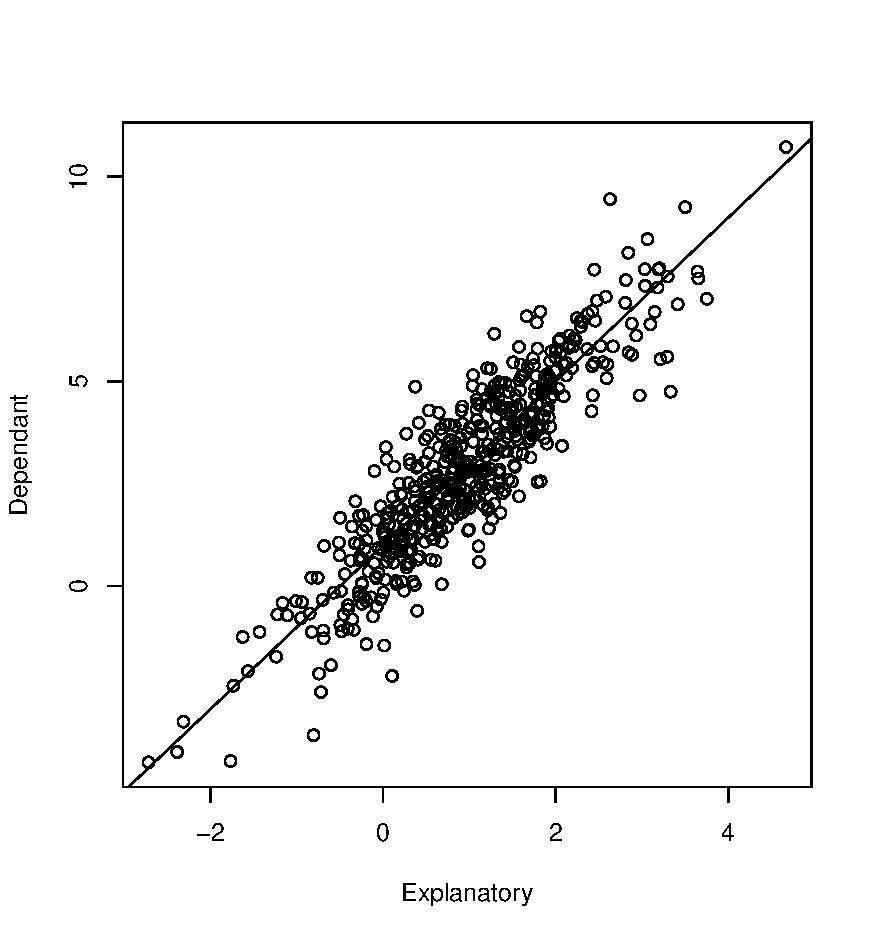
\includegraphics[width = \textwidth]{figures/Rplot05HOMONYYY.pdf}
    \caption{Homoskedasticity}
    \label{fig:homo_with_dependent_up_axis}
\end{subfigure}%
\begin{subfigure}[b]{0.5\textwidth}
\centering
    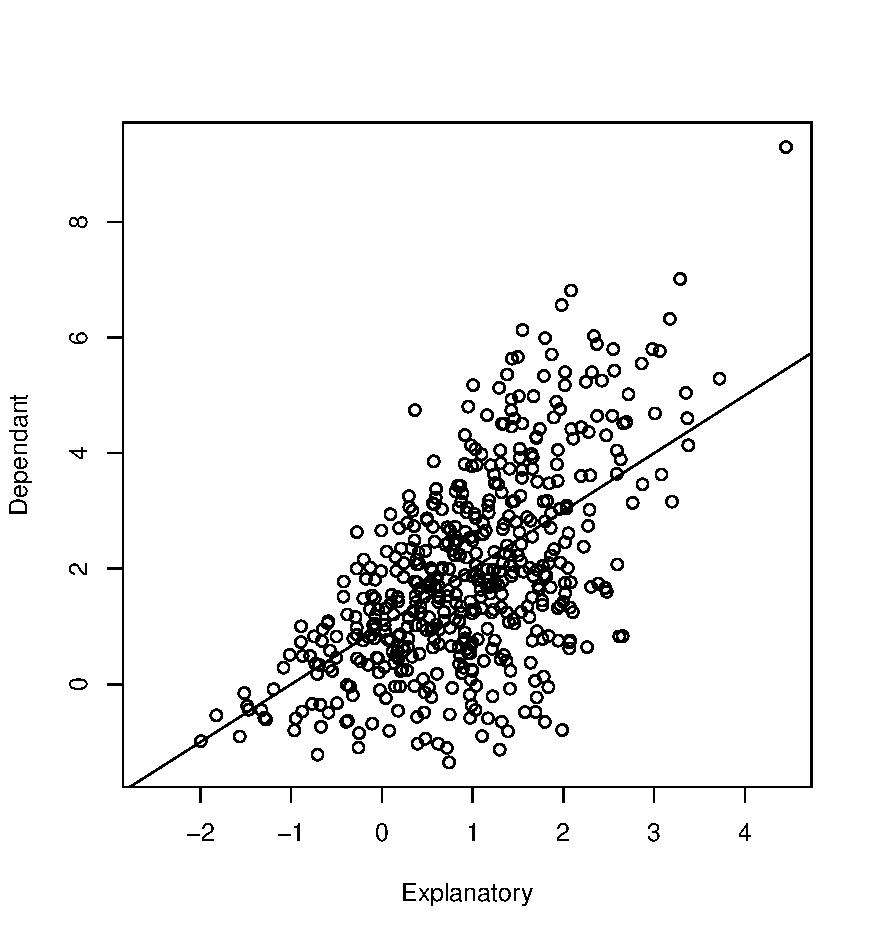
\includegraphics[width = \textwidth]{figures/Rplot05HETERONYYYY.pdf}
    \caption{Heteroskedasticity}
    \label{fig:hetero_with_dependent_up_axis}
\end{subfigure}
\end{figure}
In the case of \homo  the variance is consistent for all values of $\mathbf{X}$, so the errors do not depend on the explanatory variables.
In the case of \hetero the variance changes as the explanatory variables changes. 

For an example you can consider a households income and its spending on luxury items. If the income is low most will be spend on necessity items such as food. 
If the income is high there is the possibility but not the guarantee of spending more on luxury items, thus there will be a greater variance in the consumption of luxury goods in the segment with higher household income.
Heteroskedasticity can arise when variances of unobserved factors change over different segments in the sample space. 

It is desired to have \homo rather than \hetero because \hetero will cause problems in statistical tests and linear regression, which will be investigated further in section \ref{sec:consequence_of_hetero}. 

\subsection{OLS as the Best Linear Unbiased Estimator}
Now that the ideas of homoskedasticity and heteroskedasticity have been introduced, the next Gauss-Markov assumption can be stated.
\begin{assumption}[Homoskedasticity and no Serial Correlation]\label{as:homoskedasticity_and_no_serial_correlation}
    This assumption has two parts, the first part, regarding homoskedasticity states that
    \begin{align*}
       \var(\varepsilon_i | \mathbf{X}) = \sigma^2, \quad i = 1,2, \ldots, n.
    \end{align*}
    The second part, regarding serial correlation, states that
    \begin{align*}
        \cov(\varepsilon_i, \varepsilon_j | \mathbf{X}) = 0, \quad \text{for all} \ i \neq j.
    \end{align*}
    In matrix form these two assumptions together become
    \begin{align*}
        \var(\boldsymbol{\varepsilon} | \mathbf{X}) = \sigma^2\mathbf{I}_{n}.
    \end{align*}
\end{assumption}

With the previous assumptions in place, we are now able to derive the variance-covariance matrix of the OLS estimator.
\begin{theorem}[Variance-Covariance Matrix of the OLS Estimator]\label{th:variance-covariance_of_the_ols_estimator}
    Under assumptions \ref{as:linear_in_the_parameters}, \ref{as:no_perfect_collinearity}, \ref{as:zero_conditional_mean} and \ref{as:homoskedasticity_and_no_serial_correlation} the conditional variance of $\betahat$ on $\mathbf{X}$ satisfies
    \begin{align*}
        \var(\betahat | \mathbf{X}) = \sigma^2(\mathbf{X}^\top\mathbf{X})^{-1}.
    \end{align*}
\end{theorem}
\begin{proof}
    From \eqref{eq:beta_hat_unbiased} we have
    \begin{align}
        \var(\betahat | \mathbf{X}) &= \var\left[ (\mathbf{X}^\top\mathbf{X})^{-1}\mathbf{X}^\top\boldsymbol{\varepsilon}|\mathbf{X} \right] \nonumber\\
        &= (\mathbf{X}^\top\mathbf{X})^{-1}\mathbf{X}^\top\left[ \var(\boldsymbol{\varepsilon} | \mathbf{X}) \right] \mathbf{X}(\mathbf{X}^\top\mathbf{X})^{-1}, \label{eq:conditional_variance_of_epsilon}
    \end{align}
    and we can now use assumption \ref{as:homoskedasticity_and_no_serial_correlation} to substitute $\var(\boldsymbol{\varepsilon}|\mathbf{X})$ for $\sigma^2 \mathbf{I}$ in \eqref{eq:conditional_variance_of_epsilon} which gives
    \begin{align*}
        \var(\betahat | \mathbf{X}) &= (\mathbf{X}^\top\mathbf{X})^{-1}\mathbf{X}^\top\sigma^2 \mathbf{I} \mathbf{X}(\mathbf{X}^\top\mathbf{X})^{-1} \\
        &= \sigma^2(\mathbf{X}^\top\mathbf{X})^{-1}\mathbf{X}^\top \mathbf{X}(\mathbf{X}^\top\mathbf{X})^{-1} \\
        &= \sigma^2(\mathbf{X}^\top\mathbf{X})^{-1}
    \end{align*}
\end{proof}

As it was explained in conjunction with definition \ref{def:minimum_mean_square_error}, on page \pageref{def:minimum_mean_square_error}, the BLUE is the estimator that has the smallest variance.
It is possible to establish conditions that any linear unbiased estimator must satisfy.
These conditions can then be used to find an expression for the variance of any linear unbiased estimator.
We can then compare the variance of the OLS estimator and the variance of any linear unbiased estimator.
This is the motivation for the following theorem, better known as the Gauss-Markov theorem.
\begin{theorem}[Gauss-Markov Theorem]
    Under assumptions \ref{as:linear_in_the_parameters}, \ref{as:no_perfect_collinearity}, \ref{as:zero_conditional_mean} and \ref{as:homoskedasticity_and_no_serial_correlation} 
    \begin{align}\label{eq:betahat_y}
        \betahat &= (\mathbf{X}^\top\mathbf{X})^{-1}\mathbf{X}^\top\mathbf{y}
    \end{align}
    is the best linear unbiased estimator for $\betabold$ \cite[p. 811]{Wooldridge2012}.
    \label{th:gauss_markoc_theorem}
\end{theorem}
\begin{proof}
    Any linear estimator $\betahat$ can be written as
    \begin{align}\label{eq:any_linear_operator}
        \boldsymbol{\Tilde{\beta}} = \mathbf{A}^\top \mathbf{y},
    \end{align}
    where $\mathbf{A}$ is an $n \times (k + 1)$ matrix.
    For the linear estimator to be unbiased conditional on $\mathbf{X}$ it must satisfy
    \begin{align}\label{eq:condition_of_unbiasedness}
        E(\betatilde|\mathbf{X}) = \boldsymbol{\beta}.
    \end{align}
    Following that $\mathbf{y} = \mathbf{X}\boldsymbol{\beta} + \boldsymbol{\varepsilon}$ the expectation of $\betatilde$ conditional on $\mathbf{X}$ can be written as
    \begin{align}
       E(\betatilde|\mathbf{X}) &= E( \mathbf{A}^\top\mathbf{X}\boldsymbol{\beta} + \mathbf{A}^\top\boldsymbol{\varepsilon}|\mathbf{X} )\nonumber \\
        &=  \mathbf{A}^\top\mathbf{X}\boldsymbol{\beta} + E( \mathbf{A}^\top\boldsymbol{\varepsilon}|\mathbf{X} )\nonumber \\
        &=\mathbf{A}^\top\mathbf{X}\boldsymbol{\beta} +  \mathbf{A}^\top E( \boldsymbol{\varepsilon}|\mathbf{X} )\nonumber \\
        &=\mathbf{A}^\top\mathbf{X}\boldsymbol{\beta}\label{eq:expectation_of_any_linear_unbiased_estimator}
    \end{align}
    For the linear estimator to be unbiased it must be that \eqref{eq:expectation_of_any_linear_unbiased_estimator} is equal to the right side of \eqref{eq:condition_of_unbiasedness}, as below
    \begin{align}\label{eq:unbiasedness_identity}
        \mathbf{A}^\top\mathbf{X}\boldsymbol{\beta} = \boldsymbol{\beta}
    \end{align}
    The relation in \eqref{eq:unbiasedness_identity} holds if and only if $\mathbf{A}^\top\mathbf{X} = \mathbf{I}_{k + 1}$, which furthermore implies that $(\mathbf{A}^\top\mathbf{X})^\top = \mathbf{X}^\top\mathbf{A} = \mathbf{I}_{k + 1}$.
    The variance of $\betatilde$ conditional on $\mathbf{X}$ is given by
    \begin{align}
        \var(\betatilde|\mathbf{X}) &= \var(\mathbf{A}^\top\mathbf{X}\boldsymbol{\beta} + \mathbf{A}^\top\boldsymbol{\varepsilon}|\mathbf{X}) \nonumber\\
        &= \var(\mathbf{A}^\top\mathbf{X}\boldsymbol{\beta}|\mathbf{X}) + \var(\mathbf{A}^\top\boldsymbol{\varepsilon}|\mathbf{X}) + 2 \cov\left(\mathbf{A}^\top\mathbf{X}\boldsymbol{\beta},\mathbf{A}^\top\boldsymbol{\varepsilon}|\mathbf{X}\right) \nonumber\\
        &= \var(\mathbf{A}^\top\boldsymbol{\varepsilon}|\mathbf{X}) \nonumber\\
        &= \mathbf{A}^\top\var(\boldsymbol{\varepsilon}|\mathbf{X})\mathbf{A}.\label{eq:variance_of_betatilde_conditional_on_x}
    \end{align}
    From assumption \ref{as:homoskedasticity_and_no_serial_correlation} and \eqref{eq:variance_of_betatilde_conditional_on_x} we conclude that
    \begin{align}
        \var(\betatilde|\mathbf{X}) = \sigma^2\mathbf{A}^\top\mathbf{A}
    \end{align}
    Knowing the variance of any linear unbiased estimator we can now subtract the known variance of the OLS estimator, which was found in theorem \ref{th:variance-covariance_of_the_ols_estimator}
    \begin{align}
        \var(\betatilde|\mathbf{X}) - \var(\betahat|\mathbf{X}) &= \sigma^2\mathbf{A}^\top\mathbf{A} - \sigma^2(\mathbf{X}^\top\mathbf{X})^{-1} \nonumber \\
        &= \sigma^2\left[\mathbf{A}^\top\mathbf{A} - (\mathbf{X}^\top\mathbf{X})^{-1} \right] \label{eq:subtraction_of_variances1} \\
        &= \sigma^2\left[\mathbf{A}^\top\mathbf{A} - \mathbf{A}^\top\mathbf{X}(\mathbf{X}^\top\mathbf{X})^{-1}\mathbf{X}^\top\mathbf{A} \right] \label{eq:subtraction_of_variances2} \\
        &= \sigma^2\mathbf{A}^\top\left[\mathbf{I} - \mathbf{X}(\mathbf{X}^\top\mathbf{X})^{-1}\mathbf{X}^\top \right]\mathbf{A}.\label{eq:subtraction_of_variances3}
    \end{align}
    Going from \eqref{eq:subtraction_of_variances1} to \eqref{eq:subtraction_of_variances2} we use the fact that $\mathbf{A}^\top\mathbf{X} = \mathbf{X}^\top\mathbf{A} = \mathbf{I}_{k+1}$.
    Let 
    \begin{align}\label{eq:projection_matrix}
    \mathbf{H} = \mathbf{X}(\mathbf{X}^\top\mathbf{X})^{-1}\mathbf{X}^\top,
    \end{align}
    and notice that
    \begin{align*}
        \left(\mathbf{I} - \mathbf{H}\right)^\top &= (\mathbf{I} - \mathbf{X}(\mathbf{X}^\top\mathbf{X})^{-1}\mathbf{X}^\top)^\top 
        = (\mathbf{I})^\top - \left(\mathbf{X}^\top\right)^\top\left[(\mathbf{X}^\top\mathbf{X})^{-1}\right]^\top\mathbf{X}^\top \\
        &= \mathbf{I} - \left(\mathbf{X}^\top\right)^\top\left[(\mathbf{X}^\top\mathbf{X})^{-1}\right]^\top\mathbf{X}^\top
        = \mathbf{I} - \mathbf{X}\left[(\mathbf{X}^\top\mathbf{X})^\top\right]^{-1}\mathbf{X}^\top \\
        &= \mathbf{I} - \mathbf{X}\left[\mathbf{X}^\top\left(\mathbf{X}^\top\right)^\top\right]^{-1}\mathbf{X}^\top 
        = \mathbf{I} - \mathbf{X}\left(\mathbf{X}^\top\mathbf{X}\right)^{-1}\mathbf{X}^\top = \left(\mathbf{I} - \mathbf{H}\right),
    \end{align*}
    showing that $\mathbf{H}$ is symmetric.
    Notice also that
    \begin{align*}
        \left(\mathbf{I} - \mathbf{H}\right)^2 &= \left(\mathbf{I} - \mathbf{H}\right)^\top\left(\mathbf{I} - \mathbf{H}\right) = (\mathbf{I} - \mathbf{X}\left(\mathbf{X}^\top\mathbf{X}\right)^{-1}\mathbf{X}^\top)(\mathbf{I} - \mathbf{X}\left(\mathbf{X}^\top\mathbf{X}\right)^{-1}\mathbf{X}^\top) \\
        &= \mathbf{I} - 2\mathbf{X}\left(\mathbf{X}^\top\mathbf{X}\right)^{-1}\mathbf{X}^\top + \mathbf{X}\left(\mathbf{X}^\top\mathbf{X}\right)^{-1}\mathbf{X}^\top\mathbf{X}\left(\mathbf{X}^\top\mathbf{X}\right)^{-1}\mathbf{X}^\top \\
        &= \mathbf{I} - 2\mathbf{X}\left(\mathbf{X}^\top\mathbf{X}\right)^{-1}\mathbf{X}^\top + \mathbf{X}\left(\mathbf{X}^\top\mathbf{X}\right)^{-1}\mathbf{X}^\top = \left(\mathbf{I} - \mathbf{H}\right)
    \end{align*}
    showing that $\left(\mathbf{I} - \mathbf{H}\right)$ is idempotent.
    As $\left(\mathbf{I} - \mathbf{H}\right)$ is both symmetric and idempotent it is called a projection matrix.
    Using $\left(\mathbf{I} - \mathbf{H}\right)$ and \eqref{eq:subtraction_of_variances3} we can write
    \begin{align}\label{eq:positive_semi_definite_subtraction}
        \var(\betatilde|\mathbf{X}) - \var(\betahat|\mathbf{X}) &= \sigma^2\mathbf{A}^\top\left(\mathbf{I} - \mathbf{H}\right)\mathbf{A}.
    \end{align}
    As $\left(\mathbf{I} - \mathbf{H}\right)$ is a projection matrix we can now show that \eqref{eq:positive_semi_definite_subtraction} is positive semi definite using first idempotence and then symmetry
    \begin{align*}
        \sigma^2\mathbf{A}^\top\left(\mathbf{I} - \mathbf{H}\right)\mathbf{A} &= \sigma^2\mathbf{A}^\top\left(\mathbf{I} - \mathbf{H}\right)^2\mathbf{A} = \sigma^2\mathbf{A}^\top\left(\mathbf{I} - \mathbf{H}\right)^\top\left(\mathbf{I} - \mathbf{H}\right)\mathbf{A}\\
        &= \sigma^2\left[\left(\mathbf{I} - \mathbf{H}\right)\mathbf{A}\right]^\top\left(\mathbf{I} - \mathbf{H}\right)\mathbf{A} \geq 0.
    \end{align*}
    It has now been shown that the variance of any linear unbiased operator is greater than or equal to the variance of the OLS estimator, or in other words the OLS estimator is the BLUE.
\end{proof}

% \subsection{Consequences of Heteroscedasticity}
% In this sections we wish to determine how \hetero will affect both OLS, \textit{t-statistics}, \textit{F-statistics} and \textit{confidence intervals}. 

% First we wish to determine if the estimator $\betahat$ is unbiased or biased in the presence of heteroskedasticity.  

% Remember assumption \ref{as:linear_in_the_parameters}, \ref{as:no_perfect_collinearity} and \ref{as:zero_conditional_mean}. If these hold theorem \ref{th:unbiasedness_of_ols} proved that the OLS estimator $\betahat$ is unbiased for $\boldsymbol{\beta}$, which is the same as $E[\hat{\beta}_j] = \beta_j
% $ for $j = 1,2, \ldots, k$. 

% Because the error terms in $\var(\boldsymbol{\varepsilon} | \mathbf{X})$ did no determine whether the OLS was biased or unbiased in the theorem and its proof, the presence of \hetero will not cause $\betahat$ to be biased. 

% Next we wish to determine how our measure-of-fit test $\mathcal{R}^2$ is influenced by \hetero. 
% $\mathcal{R}^2$ measures how much of the variance in the dependent variable is explained by the independent variables. In our model it determines how much of the variance in $y$ is explained in the variables $\mathbf{X}$. 
% Low values of $\mathcal{R}^2$ makes predictions difficult because most of the variance in $y$ is caused by unobserved factors in $\varepsilon$, so the OLS predictions will be hard to calculate given a set of explanatory variables.
% Consider the expression for $\mathcal{R}^2$
% \begin{align*}
%     \mathcal{R}^2 = 1 - \dfrac{SSR}{SST}
% \end{align*}
% Where \textbf{SSR} is the \textbf{sum of squared residuals} given as
% \begin{align*}
%     SSR \equiv \nsum \hat{\varepsilon}_i^2
% \end{align*}
% and \textbf{SST} is the \textbf{total sum of squares} given as
% \begin{align*}
%     SST \equiv \nsum (y_i - \overline{y})^2. 
% \end{align*}
% The $\mathcal{R}^2$ value is between $0$ and $1$. The closer the value is to one $1$ the more of the variance is accounted for in the explanatory variables, thus it is desireable to have an $\mathcal{R}^2$ value close to $1$.
% This coefficient of determination can be changed to the adjusted $\mathcal{R}^2$ as
% \begin{align*}
%     \mathcal{R}^2_{Adj} = 1 - \dfrac{SSR/(n - k - 1)}{SST/(n - 1)}
% \end{align*}
% This rewriting of the model adjusts for the number of predictors in the model. This $\mathcal{R}^2$ in- and decreases if a predictor improves more or less than expected, respectively. 

% Both SSR and SST are unconditional variances in $\mathcal{R}^2$, thus they are not influenced by the presence of \hetero.  

% This means that \hetero does not cause the OLS estimators to be biased or inconsistent and nor does it affect the $\mathcal{R}^2$ test, however it will cause the variance of the OLS estimators, i.e. $\var(\betahat)$, to be biased, which will be explained next.  

% The \homo assumption is $\var(\boldsymbol{\varepsilon} | \mathbf{X}) = \sigma^2$. If assumption \ref{as:linear_in_the_parameters}, \ref{as:no_perfect_collinearity}, \ref{as:zero_conditional_mean} and \ref{as:homoskedasticity_and_no_serial_correlation} hold the variance of the OLS estimator can be expressed as in theorem \ref{th:variance-covariance_of_the_ols_estimator}, which implies that variance of $\betahat$ given the explanatory variables has an explicit form given as
% \begin{align*}
%     \var(\betahat | \mathbf{X}) = \sigma^2(\mathbf{X}^\top\mathbf{X})^{-1}.
% \end{align*}
% The slope coefficients can be defined as 
% \begin{align}\label{eq:slope_variance_OLS_estimator}
%     \var(\hat{\beta}_j|\mathbf{X}) = \dfrac{\sigma^2}{SST_j(1- \mathcal{R}_j^2)}
% \end{align}
% Where $j = 1, \ldots, k$ and $SST_j = \nsum (x_{ij} - \overline{x}_j)^2$ is the total sample variation in $x_j$ and $\mathcal{R}^2_j$ is found from a regression on $x_j$ with all other independent variables. 

% Equation \eqref{eq:slope_variance_OLS_estimator} depends on $\sigma^2$, $SST_j$ and $\mathcal{R}^2_j$.
% Here $\sigma^2$ is an unknown variable, the larger $\sigma^2$ the larger are the variances for the OLS estimators. $SST_j$ is the total sample variation in $x_j$, the larger it is the smaller will the variance of the OLS estimators be so it is preferred to have as much sample variation as possible which can be obtained by increasing sample size. 
% Notice that $\mathcal{R}^2_j$ is found with a regression involving only the independent variables in the original model, where $x_j$ is the dependent variable. This differs from the $\mathcal{R}^2$ found by regression on $y$ with $x_1, \ldots, x_k$ as the independent variables. 
% Consider the example $y = \betahat_0 + \betahat_1 x_1 + \betahat_2 x_2 + \varepsilon$, here $\mathcal{R}^2_1$ is found by making a regression of $x_1$ on $x_2$. 
% As always an $\mathcal{R}^2_1$ value close to one means that $x_2$ explains much of the variation in $x_1$, so a value close to $1$ means that $x_1$ and $x_2$ are highly correlated.
% $\mathcal{R}^2_j$ tests how much of the variation in one of the independent variables is explained from the remaining independent variables.
% The best estimator for $\betahat_j$ is found with a low value of $\mathcal{R}^2_j$, thus a smaller relationship between the explanatory variables is desired when retrieving $\var(\betahat_j)$. Note $\mathcal{R}^2$ cannot equal $0$ due to assumption \ref{as:no_perfect_collinearity}. 

% From \eqref{eq:slope_variance_OLS_estimator} it is possible to find the standard deviation of $\betahat_j$, which is the squre root of \ref{eq:slope_variance_OLS_estimator}, which is
% \begin{align}\label{eq:standard_deviation}
%     sd(\betahat_j) = \dfrac{\sigma}{SST_j(\big(1- \mathcal{R}_j^2)\big)^{1/2}}
% \end{align}
% The standard deviation, $\sigma$, is replaced by its estimate to obtain the standard error
% \begin{align}\label{eq:standad_error}
%     se(\betahat_j) = \dfrac{\hat{\sigma}}{SST_j(\big(1- \mathcal{R}_j^2)\big)^{1/2}}
% \end{align}
% Note that the standard deviation measures the dispersion a data set has from the mean, whereas the standard errors measures how far the sample mean of the data is likely to be from the true sample space mean. 

% Since \eqref{eq:standad_error} is obtained from \eqref{eq:slope_variance_OLS_estimator}, which relies on \homo the standard error will not be a valid estimator of the standard deviation in \eqref{eq:standard_deviation} in the presence of \hetero. This means that \hetero will cause bias in the $\var(\betahat_j)$ which invalidates the standard errors, $\varepsilon$. 

% Furthermore \textit{confidence intervals}, \textit{t-statistics} and \textit{F-statistics} will no longer follow a normal distribution and thus their results will be invalid when \hetero is present. 

% The OLS is the \textbf{best linear unbiased estimator (BLUE)}, if assumption  \ref{as:linear_in_the_parameters}, \ref{as:no_perfect_collinearity}, \ref{as:zero_conditional_mean} and \ref{as:homoskedasticity_and_no_serial_correlation} holds.
% In the Gauss-Markov theorem \ref{th:gauss_markoc_theorem}, it is seen that in order for the OLS to be the BLUE it is a necessary for the \homo assumption to hold true, otherwise it would not have the smallest variance of the estimators causing it to not be the best estimator.

% In addition it is possible to determine an unbiased estimator $\sigma^2$. 
% In order for $\sigma^2$ to be unbiased it must satisfy $E[\varepsilon^2] = \sigma^2$.  This is the same as $\sigma^2 = \dfrac{1}{n}\nsum \varepsilon_i^2$.
% This is not an estimator because we do not observe $\varepsilon$. Instead isolate the error term in the OLS as $\varepsilon_i = y_i - \beta_0 - \beta_1x_{i1} - \ldots - \beta_kx_{ik}$, where $\mathbf{\beta}_j$ is unknown. 
% In order to get OLS error term we must know $\mathbf{\beta}_j$, so we replace it with its estimate so
% \begin{align*}
%      \hat{\varepsilon}_i = y_i - \hat{\beta_0} - \hat{\beta_1x_{i1}} - \ldots - \hat{\beta}_kx_{ik}.
% \end{align*}
% We can now estimate $\sigma^2$ as
% \begin{align}\label{eq:OLS_estimate_sigma_i_anden}
%     \hat{\sigma}^2 &= \dfrac{\nsum \hat{\varepsilon}^2_i}{n-k-1}\nonumber \\
%     &= \dfrac{SSR}{n-k-1}
% \end{align}
% Where $n-k-1$ is the degrees of freedom in the OLS with $n$ observations and $k$ independent variables. 
% Note $n-k-1$ is the number of observations subtracted the number of estimated parameters. 
% To derive the variance-covariance matrix for the OLS estimator we need to make an assumption regarding the variance of the error term. 
% This assumption involves homoskedasticity, so to fully understand the concept it will be introduced in the following section.
% \vspace{5mm}
% \hrule
% \vspace{5mm}
\subsection{Estimating the Variance of the Error Term}
Next we are interested in quantifying the term $\sigma^2$, because $\var(\betahat|\mathbf{X})$ depends on this constant.
As previously stated $\sigma^2$ is the variance of the error term
\begin{align*}
    \sigma^2 = \var(\varepsilon_i | \mathbf{X}) =  E\left[\Big(\varepsilon_i - E(\varepsilon_i)\Big)^2 \Big| \mathbf{X}\right] = E\left[\varepsilon_i^2 | \mathbf{X} \right],
\end{align*}
the last equality holds as $E(\varepsilon_i) = 0$.
The MLE for $\sigma^2$ is given by \eqref{eq:MLE_for_sigma} and repeated below
\begin{align}\label{eq:MLE_for_sigma_omskrevet}
    \hat{\sigma}^2 &= \frac{\|\textbf{y} - \textbf{X}( \textbf{X}^\top\textbf{X} )^{-1}\textbf{X}^\top\textbf{y}\|^2}{n}
    = \dfrac{1}{n}\sum_{i=1}^n \left(y_i - \mathbf{x}_i\betahat\right)^2.
\end{align}
% it was found in chapter \ref{ch:likelihood_theory} on page \pageref{eq:MLE_for_sigma
If we by $\hat{\varepsilon}_i$ denote the $i$'th residual, then
\begin{align}\label{eq:observed_residual}
    \hat{\varepsilon}_i = y_i - \mathbf{x}_i\betahat.
\end{align}
Inserting \eqref{eq:observed_residual} into \eqref{eq:MLE_for_sigma_omskrevet} the MLE becomes
\begin{align}\label{eq:valid_estimate}
    \hat{\sigma}^2 = \dfrac{1}{n}\sum_{i=1}^n \hat{\varepsilon}_i^2.
\end{align}
The sum in \eqref{eq:valid_estimate} is equal to $SSR(\betahat)$ yielding a third expression for the MLE
\begin{align}
    \hat{\sigma}^2 = \frac{SSR(\betahat)}{n}.
\end{align}
Regardless of the chosen expression, the MLE is a biased estimate.
% \vspace{1ex}
% \hrule
% \vspace{1ex}
% If the values of $\varepsilon_i^2$ a way to estimate the expectation of a $\varepsilon_i^2$ is to use the sample average, which in this case would be
% \begin{align}\label{eq:sample_average}
%     \dfrac{1}{n}\nsum \varepsilon_i^2.
% \end{align}
% However \eqref{eq:sample_average} is not a feasible estimator as $\varepsilon_i = y_i - \mathbf{x}_i\boldsymbol{\beta}$ is unknown to us because we do not have the true $\boldsymbol{\beta}$.
% We do however have an estimate $\betahat$ we can use to obtain an estimate for $\varepsilon_i$, lets denote the estimate
% \begin{align}\label{eq:observed_residual}
%     \hat{\varepsilon}_i = y_i - \mathbf{x}_i\betahat.
% \end{align}
% In other words this is the observed residual and it will be investigated further in section \ref{subsec:residuals}.
% We can now insert \eqref{eq:observed_residual} into \eqref{eq:sample_average} to obtain a feasible estimate for $\sigma^2$
% \begin{align}\label{eq:valid_estimate}
%     \dfrac{1}{n}\sum_{i=1}^n \hat{\varepsilon}_i^2 = \dfrac{1}{n}\sum_{i=1}^n \left(y_i - \mathbf{x}_i\betahat\right)^2 = \frac{\ssr(\betahat)}{n}.
% \end{align}
% Although the estimate \eqref{eq:valid_estimate} is valid, it turns out to be biased.
% \vspace{1ex}
% \hrule
% \vspace{1ex}
This is because the estimate does not take into account the first order conditions imposed on the residuals.
The first order conditions are the $k + 1$ equations in \eqref{eq:multiple_linear_regression_equations} on page \pageref{eq:multiple_linear_regression_equations}.
The intuition being that if we know $n - (k + 1)$ of the residuals the rest can be found using the first order conditions, which in this case becomes a system of $k + 1$ equations with $k + 1$ unknowns. 
Because of this there is only $n - (k + 1)$ degrees of freedom in the residuals compared to $n$ in the error terms \cite[p. 55]{Wooldridge2012}.
Taking this into account the unbiased estimator of $\sigma^2$ is now presented as
% \begin{align}\label{eq:sigma_hat_2_n-k-1}
%     s^2 = \frac{SSR(\betahat)}{n - (k + 1)} = \frac{SSR(\betahat)}{n - k - 1}.
% \end{align}
\begin{align}\label{eq:unbiased_variance_estimate}
    s^2 = \frac{SSR(\betahat)}{n - (k + 1)} = \frac{SSR(\betahat)}{n - k - 1}.
\end{align}
To prove that this estimator is in fact unbiased, the following theorem is presented,
% \vspace{5mm}
% \hrule
% \vspace{5mm}
\begin{theorem}[Unbiasedness of $\sigmahat$]
    Under assumptions \ref{as:linear_in_the_parameters}, \ref{as:no_perfect_collinearity}, \ref{as:zero_conditional_mean} and \ref{as:homoskedasticity_and_no_serial_correlation}, the estimator $s^2$, in \eqref{eq:unbiased_variance_estimate}, is unbiased for $\sigma^2$. This can be expressed as $E(s^2|\mathbf{X}) = \sigma^2$ for all $\sigma^2 > 0$.
\end{theorem}
\begin{proof}
    Consider the relationship $\mathbf{y} = \mathbf{X}\betahat + \boldsymbol{\hat{\varepsilon}}$.
    We start by isolating $\boldsymbol{\hat{\varepsilon}}$
    \begin{align*}
        \boldsymbol{\hat{\varepsilon}} = \mathbf{y} - \mathbf{X}\betahat.
    \end{align*}
    Now $\betahat$ can be replaced by $\left(\mathbf{X}^\top\mathbf{X}\right)^{-1}\mathbf{X}^\top\mathbf{y}$, see \eqref{eq:equation_to} on page \pageref{eq:equation_to}, and \eqref{eq:projection_matrix} can be used to rewrite the expression 
    \begin{align}
        \hat{\boldsymbol{\varepsilon}} = \mathbf{y} - \mathbf{X}\left(\mathbf{X}^\top\mathbf{X}\right)^{-1}\mathbf{X}^\top\mathbf{y}
        = \left(\mathbf{I} - \mathbf{H}\right)\mathbf{y}. \label{eq:replace_with_y}
    \end{align}
    Using the relationship stated at the beginning of this proof lets us rewrite \eqref{eq:replace_with_y} as
    \begin{align*}
        \boldsymbol{\hat{\varepsilon}} &= \left(\mathbf{I} - \mathbf{H}\right)\left(\mathbf{X}\betahat + \boldsymbol{\hat{\varepsilon}}\right) 
        = \left(\mathbf{I} - \mathbf{H}\right)\mathbf{X}\betahat + \left(\mathbf{I} - \mathbf{H}\right)\boldsymbol{\hat{\varepsilon}}
        = \left(\mathbf{I} - \mathbf{H}\right)\mathbf{X}\betahat + \left(\mathbf{I} - \mathbf{H}\right)\boldsymbol{\varepsilon}\\
        &= \mathbf{X}\betahat - \mathbf{H}\mathbf{X}\betahat + \boldsymbol{\varepsilon} - \mathbf{H}\boldsymbol{\varepsilon}
        = \mathbf{X}\betahat - \mathbf{X}\left(\mathbf{X}^\top\mathbf{X}\right)^{-1}\mathbf{X}^\top\mathbf{X}\betahat + \boldsymbol{\varepsilon} - \mathbf{X}\left(\mathbf{X}^\top\mathbf{X}\right)^{-1}\mathbf{X}^\top\boldsymbol{\varepsilon} \\
        &= \mathbf{X}\betahat - \mathbf{X}\betahat + \boldsymbol{\varepsilon} - \mathbf{X}\left(\mathbf{X}^\top\mathbf{X}\right)^{-1}\mathbf{X}^\top\boldsymbol{\varepsilon} 
        = \boldsymbol{\varepsilon} - \mathbf{X}\left(\mathbf{X}^\top\mathbf{X}\right)^{-1}\mathbf{X}^\top\boldsymbol{\varepsilon} = \left(\mathbf{I} - \mathbf{H}\right)\boldsymbol{\varepsilon}.
    \end{align*}
    In the third equality we use $(\textbf{I} - \textbf{H})\hat{\boldsymbol{\varepsilon}} = (\textbf{I} - \textbf{H})^\top(\textbf{I} - \textbf{H})\boldsymbol{\varepsilon} = (\textbf{I} - \textbf{H})\boldsymbol{\varepsilon}$.
    Using the same property we see that
    \begin{align*}
        \boldsymbol{\hat{\varepsilon}}^\top\boldsymbol{\hat{\varepsilon}} = \left[  \left(\mathbf{I} - \mathbf{H}\right)\boldsymbol{\varepsilon} \right]^\top\left[ \left(\mathbf{I} - \mathbf{H}\right)\boldsymbol{\varepsilon} \right] = \boldsymbol{\varepsilon}^\top\left(\mathbf{I} - \mathbf{H}\right)^\top \left(\mathbf{I} - \mathbf{H}\right)\boldsymbol{\varepsilon} = \boldsymbol{\varepsilon}^\top \left(\mathbf{I} - \mathbf{H}\right)\boldsymbol{\varepsilon}.
    \end{align*}
    Furthermore because $\boldsymbol{\varepsilon}^\top \left(\mathbf{I} - \mathbf{H}\right)\boldsymbol{\varepsilon}$ is a scalar, it is equal to its trace.
    Thus we can rewrite the expectation of $\boldsymbol{\varepsilon}^\top \left(\mathbf{I} - \mathbf{H}\right)\boldsymbol{\varepsilon}$ conditional on $\mathbf{X}$ using this fact
    % \begin{center}
    %     \titlerule
    %     \Large{\textbf{Her er nogle traceregler som jeg lige skal have kigget på, og måske skrive lidt mere ud.}}
    %     \titlerule
    % \end{center}
    \begin{align}
        E\left[\boldsymbol{\varepsilon}^\top \left(\mathbf{I} - \mathbf{H}\right)\boldsymbol{\varepsilon}|\mathbf{X}\right] &= E\left[\tr\left(\boldsymbol{\varepsilon}^\top \left(\mathbf{I} - \mathbf{H}\right)\boldsymbol{\varepsilon}\right)|\mathbf{X}\right] 
        = E\left[\tr\left(\left(\mathbf{I} - \mathbf{H}\right)\boldsymbol{\varepsilon}\boldsymbol{\varepsilon}^\top\right)|\mathbf{X}\right] \nonumber\\
        &= \tr\left[E\left(\left(\mathbf{I} - \mathbf{H}\right)\boldsymbol{\varepsilon}\boldsymbol{\varepsilon}^\top|\mathbf{X}\right)\right] 
        = \tr\left[\left(\mathbf{I} - \mathbf{H}\right)E\left(\boldsymbol{\varepsilon}\boldsymbol{\varepsilon}^\top|\mathbf{X}\right)\right] \nonumber\\
        &= \tr\left[\left(\mathbf{I} - \mathbf{H}\right)\sigma^2\mathbf{I}_{n}\right]
        = \sigma^2\tr\left[\left(\mathbf{I} - \mathbf{H}\right)\right]. \label{eq:trace_projection_matrix}
    \end{align}
    In the above computation we use the fact that the trace of a product are invariant under cyclical permutations of the factors and that the trace and expectation commutes as the trace is a linear operator. 
    Notice that the trace of $\left(\mathbf{I} - \mathbf{H}\right)$ can be rewritten as
    \begin{align*}
        \tr\left[\left(\mathbf{I}_n - \mathbf{H}\right)\right] &= \tr(\mathbf{I}_n) - \tr\left[\mathbf{X}(\mathbf{X}^\top\mathbf{X})^{-1}\mathbf{X}^\top\right] \\
        &= n - \tr\left[ (\mathbf{X}^\top\mathbf{X})^{-1}\mathbf{X}^\top\mathbf{X} \right] \\
         &= n - \tr\left[\mathbf{I}_{k + 1} \right] \\
        &= n - (k + 1) = n - k - 1.
    \end{align*}
    Therefore,
    \begin{align*}
        E\left(s^2|\mathbf{X}\right) &= \frac{E\left[SSR(\betahat)|\textbf{X}\right]}{n - k - 1} = \frac{E\left[\boldsymbol{\hat{\varepsilon}}^\top\boldsymbol{\hat{\varepsilon}}|\textbf{X}\right]}{n - k - 1}= \frac{ E\left[\boldsymbol{\varepsilon}^\top \left(\mathbf{I} - \mathbf{H}\right)\boldsymbol{\varepsilon}|\mathbf{X}\right]}{n - k - 1} \\ &= \frac{\sigma^2\tr\left[\left(\mathbf{I} - \mathbf{H}\right)\right]}{n - k - 1} = \frac{\sigma^2(n - k - 1)}{n - k - 1} = \sigma^2
    \end{align*}
    which concludes the proof c.f. definition \ref{def:Unbiased_estmator}.
\end{proof}
% During this chapter we have found that under the Gauss-Markov assumptions;
% \begin{enumerate}
%     \item Linear in parameters
%     \item No perfect collinearity
%     \item Zero conditional mean
%     \item Homoskedasticity and no serial correlation
% \end{enumerate}
%  the OLS estimator is the BLUE. 
%  In addition we have found an unbiased estimator for the variance of the error term conditional on $\textbf{X}$.